\documentclass[11pt]{article}

\usepackage[margin=1in]{geometry}
\usepackage{graphicx}
\usepackage{float}
\usepackage{enumitem}
\usepackage{hyperref}

\graphicspath{{figures/}}
\setlist{nosep}

\title{ESP32-C3 Board in KiCad}
\author{}
\date{}

\begin{document}

\maketitle

\section{Project Setup}

\begin{itemize}
  \item New KiCad Project
  \item Name $\rightarrow$ ``esp32'' in its own folder
  \item Open schematic
\end{itemize}

\section{Schematic}

\subsection{ESP32 Module}

\begin{itemize}
  \item ``a'' $\rightarrow$ add \texttt{esp32-c3-wroom-02} (onboard antenna)
\end{itemize}

\subsection{USB-C}

\begin{itemize}
  \item Add: \texttt{USB\_C\_Receptacle\_USB2.0\_16P}
  \item With footprint: \texttt{HRO\_TYPE-C-31-M-12}
  \item Add GND connection to GND and Shield
  \item Add 5.1k pull-down resistors from CC1 and CC2 to GND
  \item All resistors, capacitors and the LED use 0603 footprints:
  \begin{itemize}
    \item \texttt{Resistor\_SMD:R\_0603\_1608Metric}
    \item \texttt{Capacitor\_SMD:C\_0603\_1608Metric}
    \item \texttt{LED\_SMD:LED\_0603\_1608Metric}
  \end{itemize}
\end{itemize}

\begin{figure}[H]
  \centering
  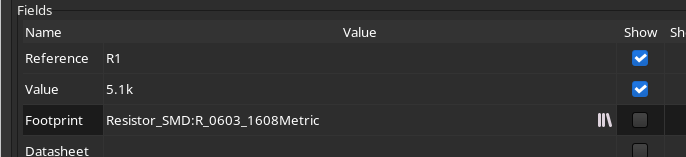
\includegraphics[width=\textwidth]{r1-fields.png}
  \caption{Fields for R1.}
  \label{fig:r1-fields}
\end{figure}

\begin{itemize}
  \item ``Q'' no connect SBU1 and SBU2
\end{itemize}

\begin{figure}[H]
  \centering
  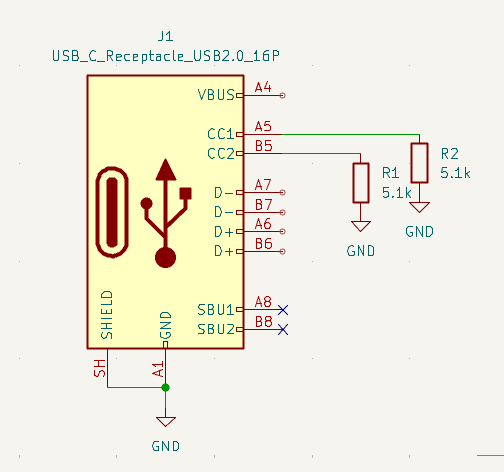
\includegraphics[width=0.6\textwidth]{usb-c.png}
  \caption{USB-C receptacle with CC pull-downs and SBU no-connects.}
  \label{fig:usb-c}
\end{figure}

\begin{itemize}
  \item +5V flag at VBUS
  \item PWR flag on +5V and GND
\end{itemize}

\subsection{Regulator}

\texttt{AP2112K-3.3}

\begin{itemize}
  \item VIN: +5V
  \item Decoupling cap 10\,\textmu F rated at 10\,V to GND
  \item Tie EN to VIN
  \item GND to GND
  \item Decoupling cap 10\,\textmu F rated at 10\,V to VOUT
  \item VOUT to 3.3V flag
\end{itemize}

\begin{figure}[H]
  \centering
  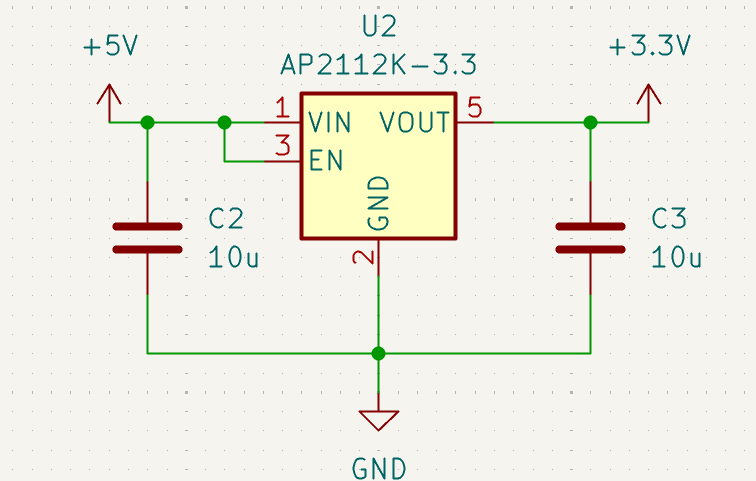
\includegraphics[width=0.6\textwidth]{regulator.png}
  \caption{AP2112K-3.3 regulator with input and output decoupling.}
  \label{fig:regulator}
\end{figure}

\subsection{USB Data Lines}

Use ``L'' to place a Net Label.

\begin{itemize}
  \item D$-$ tied together
  \item D$-$ is USB$-$
  \item D+ tied together
  \item D+ is USB+
\end{itemize}

\begin{figure}[H]
  \centering
  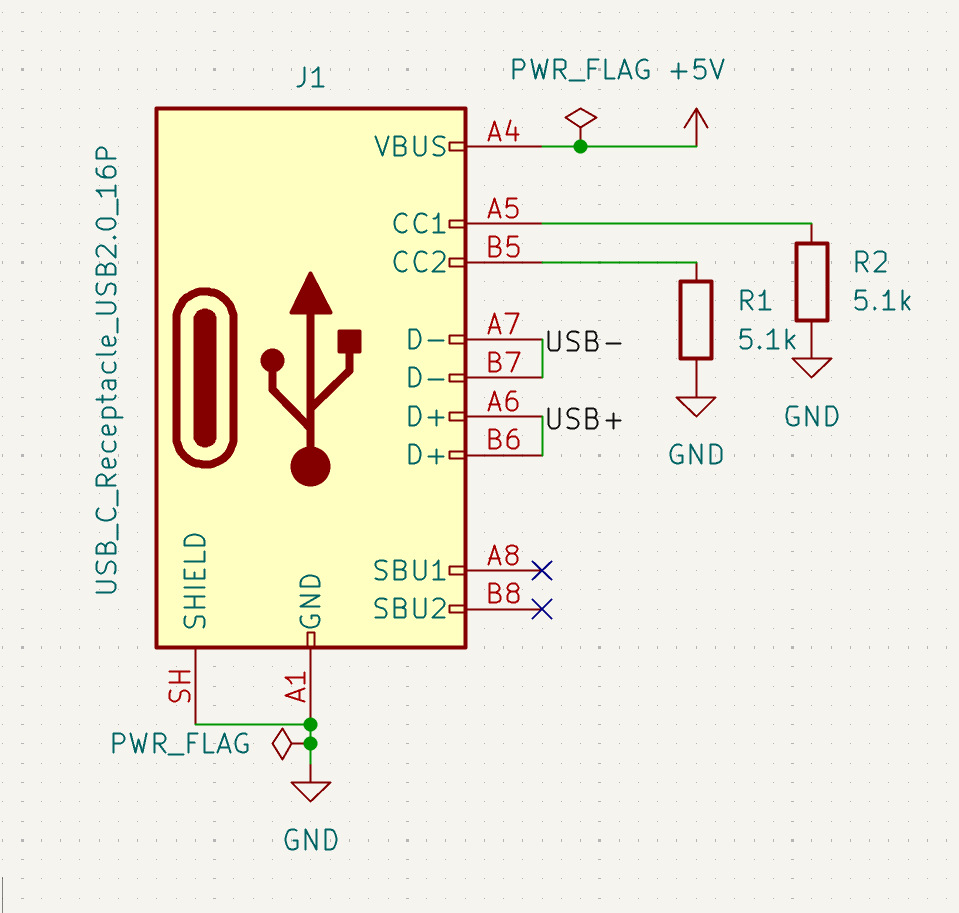
\includegraphics[width=0.6\textwidth]{usb-c-complete.png}
  \caption{Completed USB-C connector.}
  \label{fig:usb-c-complete}
\end{figure}

\subsection{Button}

\begin{itemize}
  \item Button: \texttt{SW\_Push}
  \item Button footprint: \texttt{Button\_Switch\_SMD:SW\_SPST\_PTS810}
\end{itemize}

\subsection{ESP32 Decoupling}

\begin{itemize}
  \item 3.3V to 3V3
  \item Add 0.1\,\textmu F to GND, 16\,V rated
  \item Add 10\,\textmu F to GND, 16\,V too
  \item Pull up 10k from EN to 3.3V
  \item Add decoupling cap 1\,\textmu F to EN
  \item IO9: pull up 10k to 3.3V
  \item Add switch to GND
\end{itemize}


\subsection{I2C}

\begin{itemize}
  \item 4.7k pull-up to 3.3V on pins 2 and 8
  \item SDA: IO2
  \item SCL: IO8
\end{itemize}

\subsection{Status LED}

\begin{itemize}
  \item IO10 $\rightarrow$ 1\,k$\Omega$ resistor $\rightarrow$ 0603 LED
    $\rightarrow$ GND
\end{itemize}

\begin{figure}[H]
  \centering
  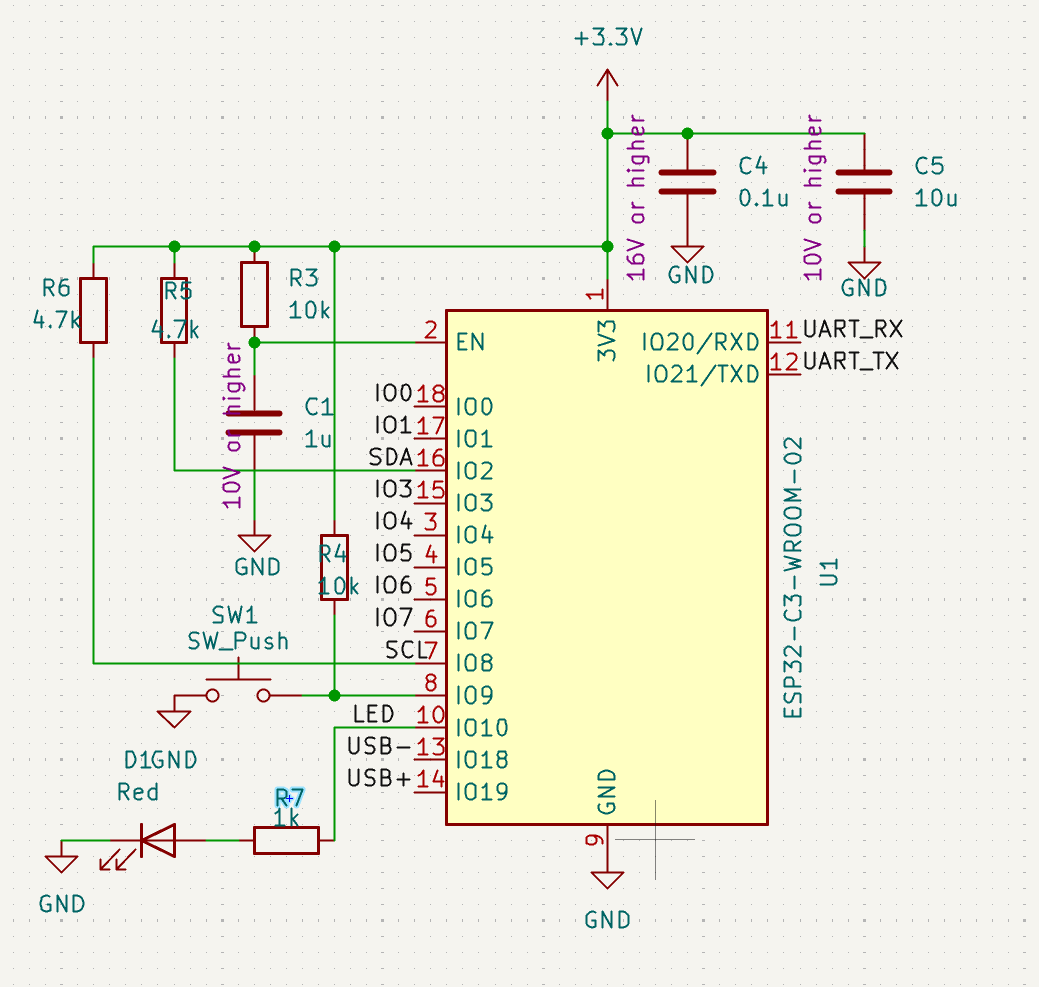
\includegraphics[width=0.85\textwidth]{esp32-module.png}
  \caption{ESP32-C3 module with decoupling, EN, boot button, I2C pull-ups and status LED.}
  \label{fig:esp32-module}
\end{figure}

\begin{figure}[H]
  \centering
  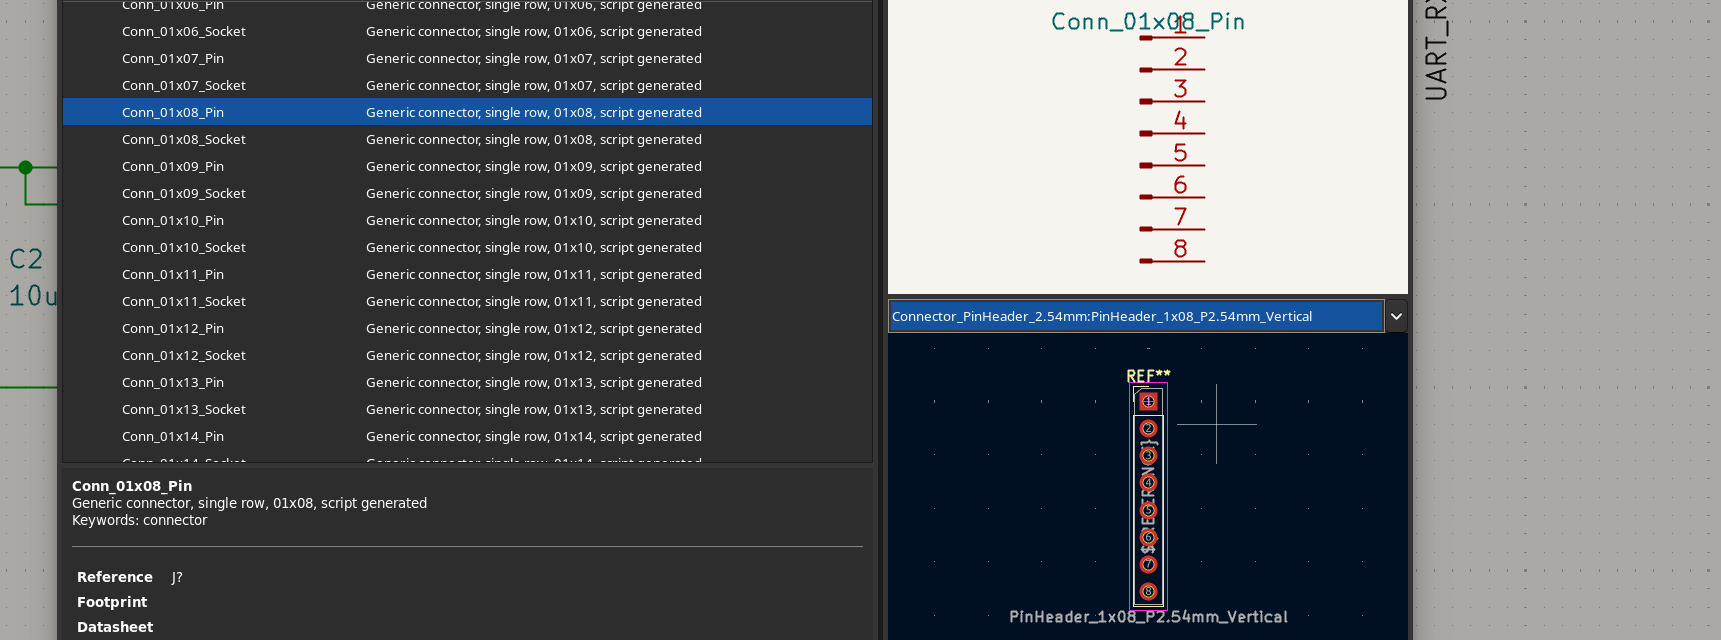
\includegraphics[width=\textwidth]{header-chooser.png}
  \caption{\texttt{Conn\_01x08\_Pin} with footprint
    \texttt{PinHeader\_1x08\_P2.54mm\_Vertical}.}
  \label{fig:header-chooser}
\end{figure}

\begin{figure}[H]
  \centering
  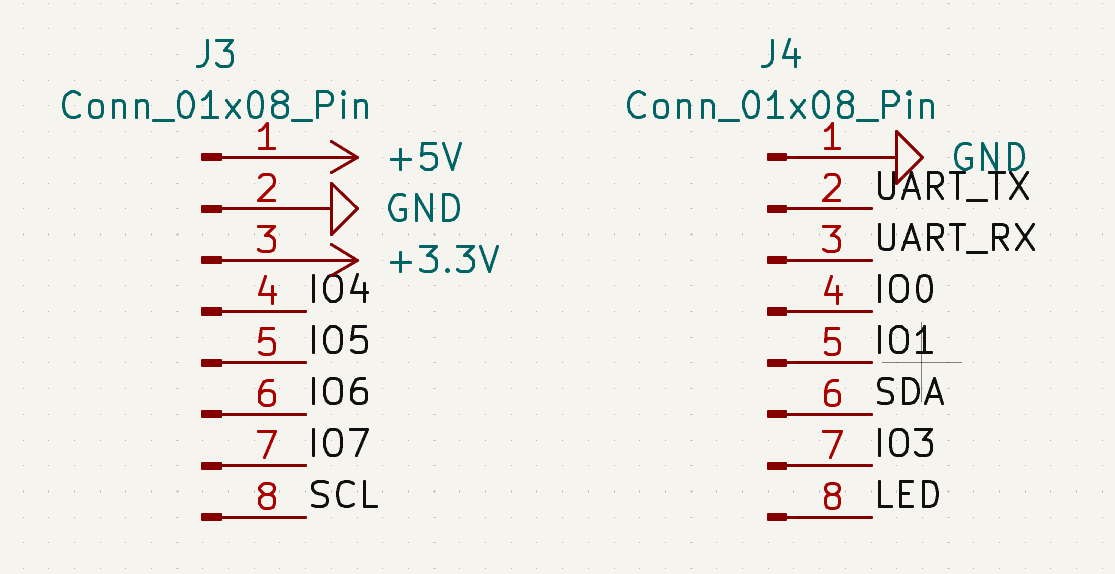
\includegraphics[width=0.6\textwidth]{headers.png}
  \caption{J3 and J4 pin headers.}
  \label{fig:headers}
\end{figure}

\begin{itemize}
  \item J3 (left side of U1): +5V, GND, +3.3V, IO4, IO5, IO6, IO7, SCL
  \item J4 (right side of U1): GND, UART\_TX, UART\_RX, IO0, IO1, SDA, IO3, LED
\end{itemize}

\subsection{Checking the Schematic}

\begin{enumerate}
  \item \textbf{ERC:} Inspect $\rightarrow$ Electrical Rules Checker
    $\rightarrow$ Run ERC. Aim for zero errors, then read each warning
    instead of ignoring it.
  \item \textbf{Highlight a net:} select a wire and press \texttt{\`{}}
    (backtick) to highlight everything on that net. Click SDA and SCL in
    turn and make sure each lights up only its own pins.
\end{enumerate}

\section{PCB Editor}

\subsection{Board Setup}
\begin{enumerate}
	\item Update PCB from schematic (F8)
	\item Change grid to 0.25 mm
	\item Click the green PCB icon with the gear (Board Setup)
	\item Constraints: minimum clearance 0.15 mm, minimum track width
	0.15 mm, minimum via diameter 0.6 mm, copper to edge 0.3 mm
	(Figure~\ref{fig:constraints})
	\item Net Classes: add a \texttt{Power} class with 0.5 mm track width.
	Leave \texttt{Default} at 0.25 mm tracks, 0.6/0.3 mm vias, 0.2 mm
	differential pair width and 0.25 mm gap (Figure~\ref{fig:netclasses})
	\item Netclass Assignments: set \texttt{+5V}, \texttt{+3.3V} and
	\texttt{GND} to \textbf{Power} (the screenshot still shows Default)
	\item Pre-defined Sizes: tracks 0.25 mm and 0.5 mm, via 0.6 mm with
	0.3 mm hole (Figure~\ref{fig:screenshot002})
\end{enumerate}

\begin{figure}[H]
  \centering
  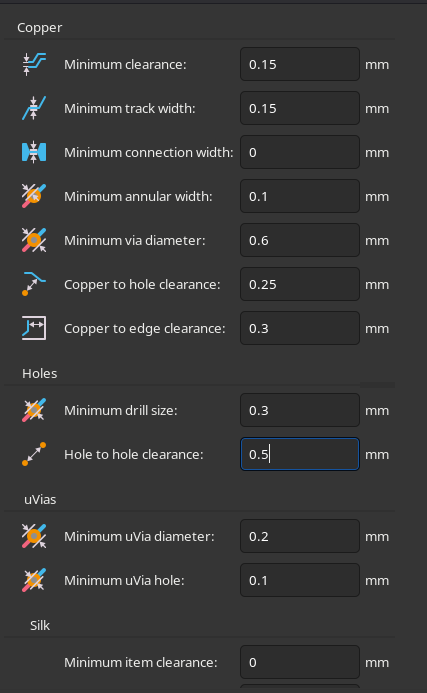
\includegraphics[width=0.55\textwidth]{constraints.png}
  \caption{Board Setup $\rightarrow$ Design Rules $\rightarrow$ Constraints.}
  \label{fig:constraints}
\end{figure}

\begin{figure}[H]
  \centering
  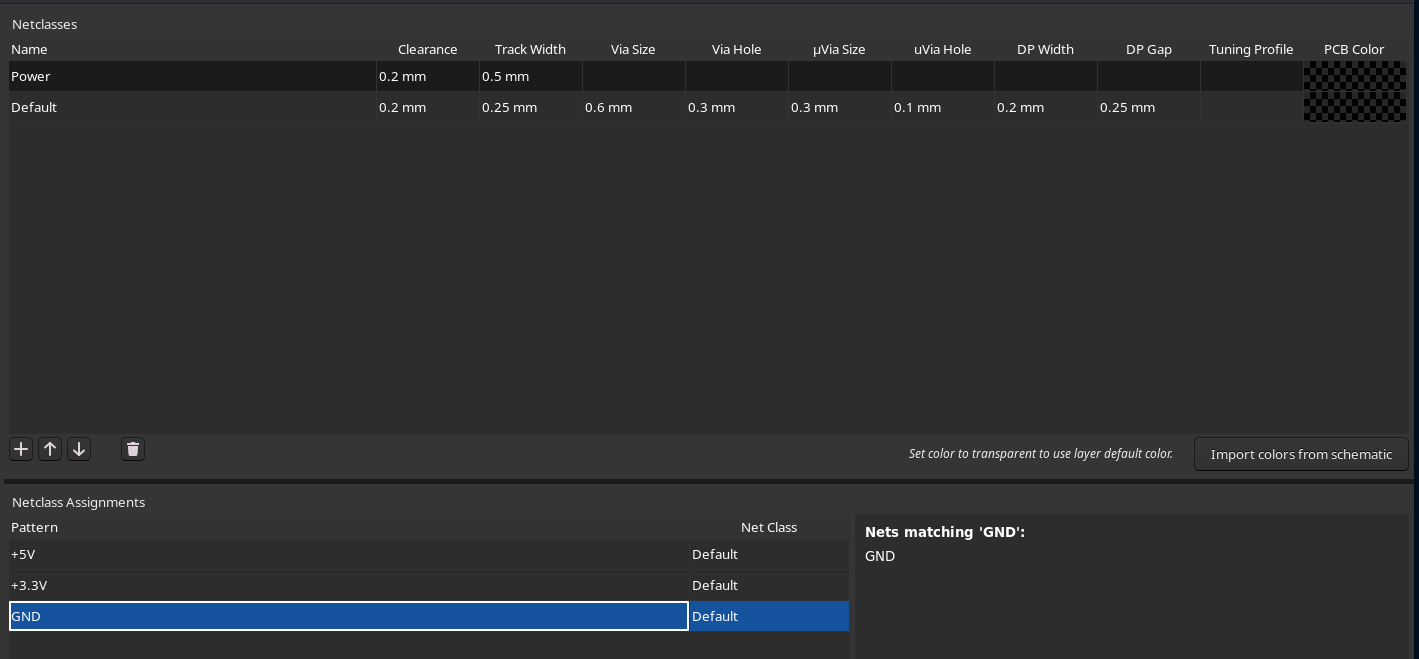
\includegraphics[width=\textwidth]{netclasses.png}
  \caption{Board Setup $\rightarrow$ Design Rules $\rightarrow$ Net Classes.}
  \label{fig:netclasses}
\end{figure}

\begin{figure}[H]
	\centering
	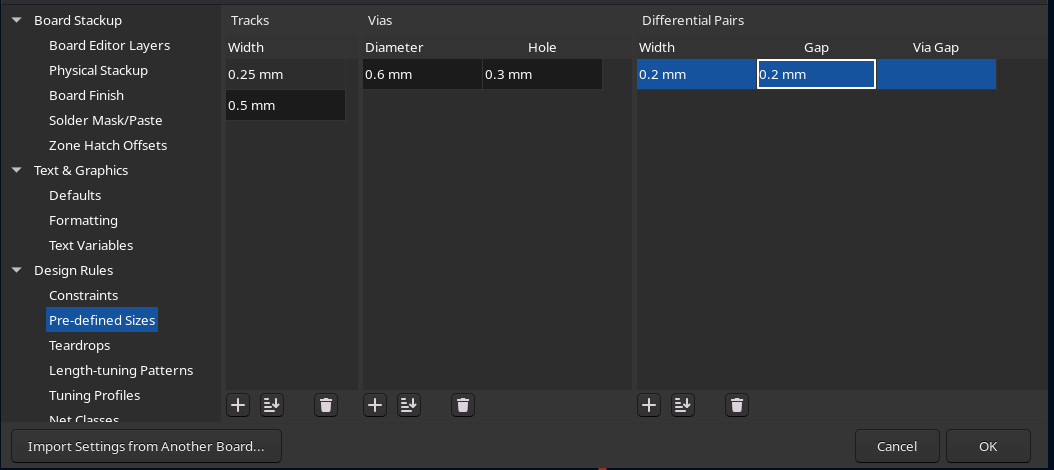
\includegraphics[width=0.7\linewidth]{figures/screenshot002}
	\caption{Board Setup $\rightarrow$ Design Rules $\rightarrow$ Pre-defined Sizes.}
	\label{fig:screenshot002}
\end{figure}

\subsection{Edge cuts}
\begin{enumerate}
	\item Select Edge.Cuts under Appearance on the right side
	\item Draw Rectangles
	\item Double-click the rectangle and set size to 50x40 mm
	\item Ctrl + Shift + M is the measure tool
\end{enumerate}

\subsection{Placement}
\begin{enumerate}
	\item Place U1 with the antenna hanging over the top board edge
	\item Keep the antenna keep-out clear of copper and parts on both layers
	\item Place J3 and J4 on a 2.54 mm grid along the left and right edges
	\item Place J1 at the bottom edge so a cable can reach it
	\item Lock U1, J1, J3 and J4 (select, then L)
	\item C4 and C5 right next to U1 pin 1 (3V3)
	\item C1 next to U1 pin 2 (EN)
	\item C2 next to U2 VIN, C3 next to U2 VOUT
	\item R1 and R2 next to the CC pins on J1
	\item R3 to R6 between the headers and U1
	\item R7 and D1 near the bottom edge so the LED is visible
	\item SW1 near the bottom edge so it is easy to press
\end{enumerate}

\begin{figure}[H]
	\centering
	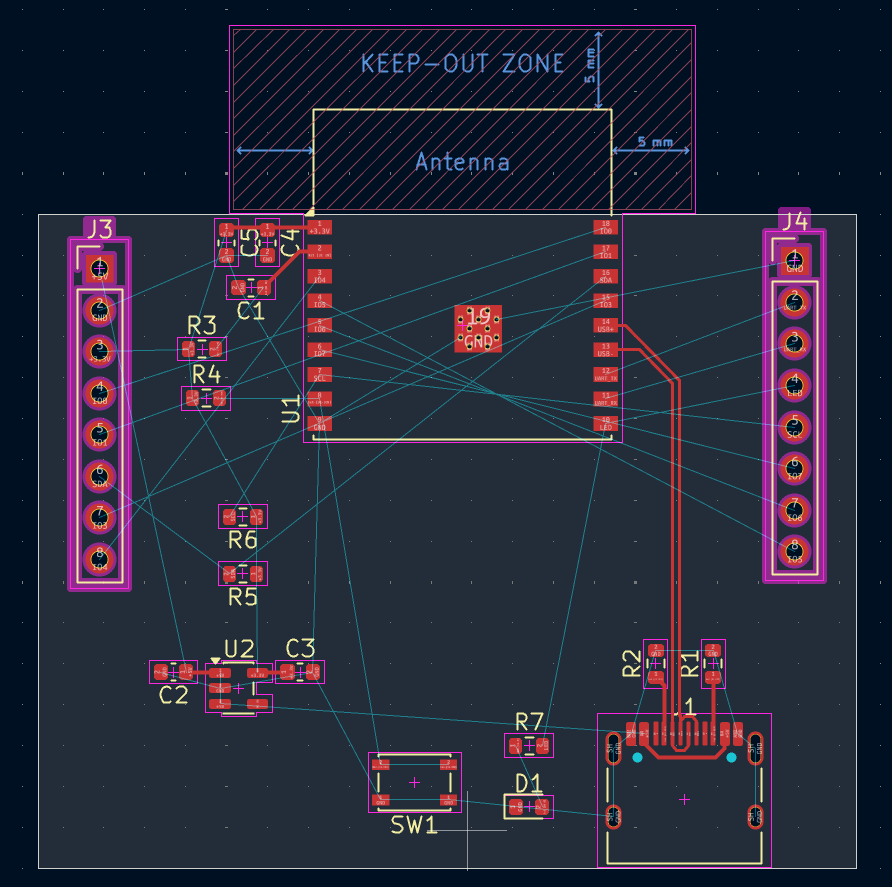
\includegraphics[width=0.85\linewidth]{placement.png}
	\caption{Placement with the USB pair routed.}
	\label{fig:placement}
\end{figure}

\subsection{Differential Router}
\begin{itemize}
	\item Press 6
	\item Click a USB+ or USB$-$ pad on J1
	\item Route to U1 pins 13 and 14 on F.Cu
	\item No vias and nothing crossing the pair
	\item Join A6 to B6 and A7 to B7 at the connector
\end{itemize}

\subsection{Routing}
\begin{enumerate}
	\item Press X to route a single track; the width follows the net class
	\item Route power (+5V, +3.3V) first: J1 VBUS $\rightarrow$ C2
	$\rightarrow$ U2 VIN, then U2 VOUT $\rightarrow$ C3 $\rightarrow$ C4/C5
	$\rightarrow$ U1 pin 1
	\item Then EN, IO9, I2C, the LED and the header pins
	\item Keep tracks on F.Cu where possible; use a via (V while routing)
	only to hop over another track
	\item Leave GND pins unrouted; the pour and stitching vias connect them
	\item Nothing routed under the antenna
\end{enumerate}

\subsection{Ground Pour}
\begin{enumerate}
	\item Select B.Cu under Appearance on the right side
	\item Place $\rightarrow$ Add Filled Zone (Ctrl + Shift + Z)
	\item Click the first corner of the board outline
	\item In the zone dialog:
	\begin{itemize}
		\item Check B.Cu and F.Cu
		\item Net: GND
		\item Clearance: 0.5 mm
		\item Minimum width: 0.25 mm
		\item Pad connections: Thermal reliefs
		\item Thermal relief gap: 0.5 mm
		\item Thermal spoke width: 0.5 mm
		\item Corner smoothing: None
		\item Remove islands: Always
	\end{itemize}
	\item Click OK
	\item Click the other corners of the board outline
	\item Double-click to close the outline
	\item Press B to fill all zones
	\item Check that no copper fills the antenna keep-out
\end{enumerate}

\begin{figure}[H]
	\centering
	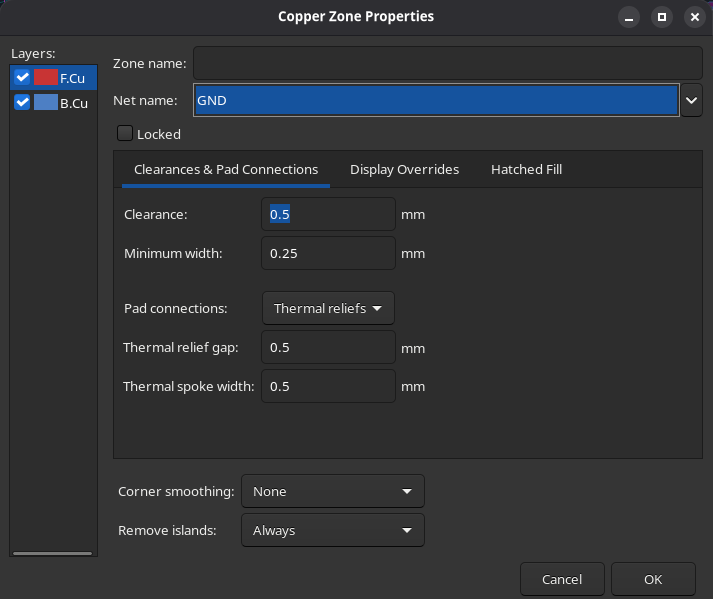
\includegraphics[width=0.7\linewidth]{zone-properties.png}
	\caption{Copper Zone Properties for the GND pour.}
	\label{fig:zone-properties}
\end{figure}

\subsection{Stitching Vias}
\begin{enumerate}
	\item Place $\rightarrow$ Add Vias (Ctrl + Shift + X)
	\item Click on the GND pour; the via takes the GND net
	\item One via every 5 to 10 mm across the board
	\item Extra vias next to each capacitor GND pad, J1 and U2
	\item 4 to 9 vias in the U1 GND pad (pin 19)
	\item Press B to refill, then run DRC
\end{enumerate}

\subsection{Design Rules Check}
\begin{enumerate}
	\item Press B to refill zones
	\item Inspect $\rightarrow$ Design Rules Checker $\rightarrow$ Run DRC
	\item Check ``Test for parity between PCB and schematic''
	\item Fix every error; zero unconnected items
	\item Click an entry to jump to it on the board
	\item Re-run until clean
\end{enumerate}

\subsection{Silkscreen}
\begin{enumerate}
	\item Move reference designators so none sit on pads or under parts
	\item Label the header pins (+5V, GND, SDA, \ldots) with Place
	$\rightarrow$ Add Text on F.SilkS
	\item Add a board name and date
	\item View $\rightarrow$ 3D Viewer (Alt + 3) to check the result
\end{enumerate}

\subsection{Fabrication Outputs}
\begin{enumerate}
	\item File $\rightarrow$ Fabrication Outputs $\rightarrow$ Gerbers
	\item Output directory: \texttt{gerbers/}
	\item Layers: F.Cu, B.Cu, F.Paste, F.SilkS, B.SilkS, F.Mask, B.Mask,
	Edge.Cuts
	\item Click Plot
	\item Click Generate Drill Files $\rightarrow$ Generate (same folder)
	\item Zip the \texttt{gerbers/} folder and upload it to the board house;
	check their Gerber preview before ordering
\end{enumerate}

\end{document}
